%!TEX root = ../../master.tex
\chapter{Experiment: Application Level and Infrastructure Level Resilience}
\label{appendix_resilience}

This appendix will present additional results from the experiments, present the students' experiments, and cover how scripts were used during the experiments. The source code and results can be found in Attachment 5 and 6. All tests were performed in a KubeCloud consisting of four Raspberry Pis as seen in Figure~\ref{fig:topology}.

\section*{Application Level Resilience Extra Results}
In addition to the scenarios presented in Chapter~\ref{chapter_experiment2_resilience} called \textit{Integration points in a synchronous architecture}, three test runs of the setup without delay and circuit breakers were performed to act as a reference point. The measurements were performed to investigate the latencies and success rates at the 100 requests per second as in the experiment. Figure~\ref{fig:appendix_no_delay} shows a normalized histogram of the three test runs.

\begin{figure}[H]
    \centering
    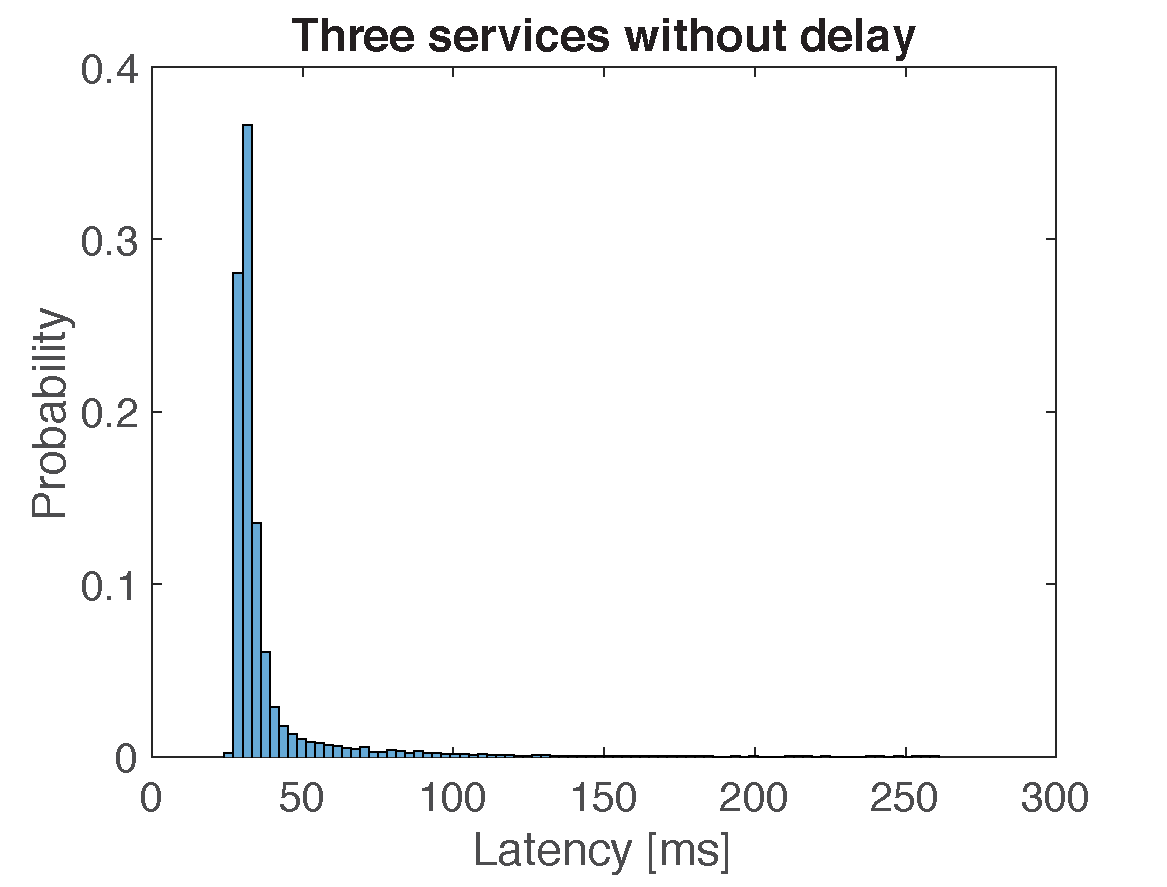
\includegraphics[width=8.5cm]{figures/appendix/no_delay}
    \caption{Test Setup without Delay}
    \label{fig:appendix_no_delay}
\end{figure}

\noindent
All test runs had 100\% success ratio and on average a response time of 36.6 ms. \\

\noindent
The source code of three services is available on Github as: lab-service-0, lab-service-1, lab-service-2 on \url{https://github.com/rpicloud/}. Docker images are available on Docker Hub as: exp-circuitbreaker-service-0, exp-circuitbreaker-service-1, and exp-circuitbreaker-service-2 tagged with version \textit{0.0.7}: \url{https://hub.docker.com/r/rpicloud/}.


\section*{Application Level Resilience Scripts}
The configuration of the circuit breakers in the three services (Service 0, Service 1, Service 2) are different in the scenarios. Vegeta was used to perform HTTP requests towards Service 0. Scripts made the process simpler and replicable. The scripts expect the host and rate as parameters, and different configurations such as delays and timeouts are configured. When the configuration is set up, a folder for output is created, the attack starts, and attack reports are generated. The line below shows how to call the script.


\begin{lstlisting}
sh two_circuit_breakers.sh --host=192.168.1.71 --rate=100
\end{lstlisting}
\noindent
Listing~\ref{lst:twocb_script} shows how the configuration, test run, and report generation for the scenario with two circuit breakers. The scripts for the three circuit breaker scenarios in Chapter~\ref{chapter_experiment2_resilience} follow the same structure. Vegeta attacks produce .bin files. Afterward, Vegeta creates reports from the .bin files. These reports have been used to output e.g. graphs and CSV files.


\lstinputlisting[language=bash,label={lst:twocb_script}, caption={Two Circuit Breakers}]{scripts/4_cb_3svc_delay.sh}

\section*{Application Level Resilience Student Experiments}
The scripts made it easy to reproduce the experiments for the students. Table~\ref{table:appendix_student_integration_points} shows the results of the students' results of the \textit{Integration points in a synchronous architecture} experiment. Tests were performed on a shared wireless router whereas our experiments were performed with an ethernet cable. By inspecting the results, it is seen that errors such as 'too many open files' occur. This probably caused extra errors and lower success rate in some of the scenarios. Group 5 had a success rate of 49.1\% whereas Group 2's success rate was 100\% with one circuit breaker. Concluding exact values from these results does not make sense due to the variation, but the success rate was improved using circuit breakers in all except one test case.

\renewcommand*{\arraystretch}{1.7}
\begin{table}[H]
\centering
\begin{tabular}{|p{2cm}|p{3.5cm}|p{3.5cm}|p{3.5cm}|} 
\hline
\rowcolor[HTML]{EFEFEF} \textbf{Success rate} &     \textbf{No circuit breaker} & \textbf{One circuit breaker} & \textbf{Two circuit breakers} \\ \hline
\textbf{Group 2} &     6.8\% & 100\% & 100\% \\ \hline
\textbf{(Extra)} &     6.9\% & 100\% & 75.77\% \\ \hline
\textbf{Group 3} &     6.67\% & 70.17\% & 79.27\% \\ \hline
\textbf{(Extra)} &     - & - & 95.67\% \\ \hline
\textbf{Group 4} &     11.73\% & 74.9\% & 100\% \\ \hline
\textbf{(Extra)} &     - & - & 98.77\% \\ \hline
\textbf{Group 5} &     12.07\% & 49.1\% & 99.53\% \\ \hline
\textbf{(Extra)} &     - & \% & 61.71\% \\ \hline
\rowcolor[HTML]{EFEFEF} \textbf{Average} &     8.83\% & 78.83\% & 92.72\% \\ \hline
\end{tabular}
\caption{Comparison of Success Rates from Student Exercises}
\label{table:appendix_student_integration_points}
\end{table}





\section*{Infrastructure Level Resilience Extra Results}

Docker images for ARM architecture can be found on Docker Hub: \url{https://hub.docker.com/r/rpicloud/greeting-rpi/}. 

\subsection*{Effects of Replication}

In experiment \textit{Recovery time} presented in Chapter~\ref{chapter_experiment2_resilience} Table~\ref{table:recovery_rates} presented the success rates for rate 100 requests/second and 200 requests/second. Table~\ref{table:appendix_recovery_time} and Table~\ref{table:appendix_recovery_time_2} shows the measurement from each iteration that Table~\ref{table:recovery_rates} is based on.
\renewcommand*{\arraystretch}{1.8}
\setlength\LTleft{0pt}
\setlength\LTright{0pt}
\begin{longtable}{@{\extracolsep{\fill}}|p{3cm}|p{2.5cm}|p{2.5cm}|p{2.5cm}|p{2.5cm}|} 
\hline
\rowcolor[HTML]{EFEFEF} \textbf{Sucess rate} & \textbf{Iteration 1} & \textbf{Iteration 2} & \textbf{Iteration 3} & \textbf{Average}\\
\hline
\endfirsthead
\multicolumn{5}{c}%
{\tablename\ \thetable\ -- \textit{Continued from previous page}} \\
\hline
\rowcolor[HTML]{EFEFEF} & \textbf{Iteration 1} & \textbf{Iteration 2} & \textbf{Iteration 3} & \textbf{Average}\\
\hline
\endhead
\hline \multicolumn{5}{r}{\textit{Continued on next page}} \\
\caption{Rate=100 (Total of 18,000 Requests)}
\endfoot
\hline
\caption{Rate=100 (Total of 18,000 Requests)}
\label{table:appendix_recovery_time}
\endlastfoot

\textbf{replicas=1} & 73.93\% (13,307/4,693) & 73.93\% (13,307/4,693) & 76.09\% (13,696/4,304) & \textbf{74.65\% (13,437/4,563)} \\ \hline
\textbf{replicas=2} & 99.89\% (17,980/20)& 99.86\% (17,975/25) & 99.87\% (17,977/23) & \textbf{99.87\% (17,977/23)} \\ \hline
\textbf{replicas=5} & 99.99\% (17,998/2) & 99.97\% (17,994/6) & 99.98\% (17,996/4)  & \textbf{99.98\% (17,996/4)} \\ \hline
\end{longtable}


\renewcommand*{\arraystretch}{1.8}
\setlength\LTleft{0pt}
\setlength\LTright{0pt}
\begin{longtable}{@{\extracolsep{\fill}}|p{3cm}|p{2.5cm}|p{2.5cm}|p{2.5cm}|p{2.5cm}|} 
\hline
\rowcolor[HTML]{EFEFEF} \textbf{Success rate} & \textbf{Iteration 1} & \textbf{Iteration 2} & \textbf{Iteration 3} & \textbf{Average}\\
\hline
\endfirsthead
\multicolumn{5}{c}%
{\tablename\ \thetable\ -- \textit{Continued from previous page}} \\
\hline
\rowcolor[HTML]{EFEFEF} \textbf{Success rate} & \textbf{Iteration 1} & \textbf{Iteration 2} & \textbf{Iteration 3} & \textbf{Average}\\
\hline
\endhead
\hline \multicolumn{5}{r}{\textit{Continued on next page}} \\
\caption{Rate=200 (total of 36,000 requests)}
\endfoot
\hline
\caption{Rate=200 (total of 36,000 requests)}
\label{table:appendix_recovery_time_2}
\endlastfoot

\textbf{replicas=1} & 74.26\% (26,735/9,265) & 71.03\% (25,569/10,431) & 72,95\% (26,262/9,738) & \textbf{72.75\% (26,189/9,811)} \\ \hline
\textbf{replicas=2} & 99.86\% (35,949/51)& 99.90\% (35,963/37) & 99.88\% (35,958/42) & \textbf{99.88\% (35,957/43)} \\ \hline
\textbf{replicas=5} & 99.99\% (35,996/4) & 99.99\% (35,998/2) & 99.97\% (35,988/12)  & \textbf{99,98\% (35,994/6)} \\ \hline
\end{longtable}



\section*{Infrastructure Level Resilience Scripts}
The scripts make the test process of the experiments simple and replicable. This ensures that the same steps are always taken during the execution of the experiments. Listing~\ref{lst:example_replicatest} shows an example of the test script for running the \textit{The effects of replication} experiment. Running the script takes the host as a parameter and can easily be directed against other hosts or clusters.
\newpage
\lstinputlisting[language=bash,label={lst:example_replicatest}, caption={Replica Test Ramp-Up}]{scripts/example_replicatest.sh}

\newpage
\section*{Infrastructure Level Resilience Student Experiments}
Because the scripts made it easy to reproduce the experiments, it was possible to use the tests as an exercise for the students. Table~\ref{table:appendix_recovery_rates} shows the results of the five groups' test results of the \textit{Recovery time} experiment. Tests were performed on a shared wireless router whereas our experiments were performed with an ethernet cable. Most of the results are very close to our experiments, but the scenario with one replica at a request rate of 100 requests/second has a success rate of 58.65\% whereas our success rate is 74.65\%. By inspecting the results, it is seen that errors such as 'too many open files' occur. This probably caused extra errors leading to a lower success rate. 

\begin{centering}
\renewcommand*{\arraystretch}{1.8}
\setlength\LTleft{0pt}
\setlength\LTright{0pt}
\begin{longtable}{|p{2cm}|p{1.8cm}|p{1.8cm}|p{1.8cm}|p{1.8cm}|p{1.9cm}|p{1.9cm}|} 
\hline
\rowcolor[HTML]{EFEFEF} \textbf{Success rate} & \textbf{1 rep. (100)} & \textbf{2 rep. (100)} & \textbf{5 rep. (100)} & \textbf{1 rep. (200)} & \textbf{2 rep. (200)} & \textbf{5 rep. (200)}  \\
\hline
\endfirsthead
\multicolumn{3}{c}%
{\tablename\ \thetable\ -- \textit{Continued from previous page}} \\
\hline
\rowcolor[HTML]{EFEFEF} \textbf{Success rate} [\% (success/error)] & \textbf{rate=100} & \textbf{rate=200} \\
\hline
\endhead
\hline \multicolumn{3}{r}{\textit{Continued on next page}} \\
\caption{Comparison of Success Rates from Student Exercises}
\endfoot
\hline
\caption{Comparison of Success Rates from Student Exercises}
\label{table:appendix_recovery_rates}
\endlastfoot

\textbf{Group 1} & 60.48    \% & 99.95\% & 99.69\% & 74.93\% & 99.97\% & 99.92\% \\ \hline
\textbf{Group 2} & 52.42\% & 100\% & 100\% & 73.97\% & 99.98\% & 100\% \\ \hline
\textbf{Group 3} & 55.68    \% & 71.76\% & 99.99\% & 73.66\% & 99.91\% & 99.98\% \\ \hline
\textbf{Group 4} &     54.97\% & 99.88\% & 99.88\% & 74.92\% & 99.92\% & 99.98\% \\ \hline
\textbf{Group 5} &     69.68\% & 99.96\% & 99.97\% & 70.71\% & 99.85\% & 99.97\% \\ \hline
\rowcolor[HTML]{EFEFEF}  \textbf{Average} &     58.65\% & 94.31\% & 99.91\% & 73.64\% & 99.93\% & 99.97\% \\ \hline
                                
\end{longtable}
\end{centering}

